% \documentclass[10pt,a4paper]{article}
\usepackage{CJKutf8}
\renewcommand{\tablename}{表}
\usepackage{geometry}
\usepackage{graphicx}
\usepackage{float}
\usepackage{multicol}
%\usepackage{tcolorbox}
%\tcbuselibrary{skins,breakable,raster}
\usepackage{array}
%\tcbset{fonttitle=\bfseries,breakable,
%	colback=white,
%	every box/.style={enhanced,
%		before=\par\smallskip,after=\par\smallskip},
%	every box on layer 2/.style={reset,every box,colback=yellow!10!white,
%		drop fuzzy shadow}}

\geometry{left=1cm,right=1cm,top=1cm,bottom=1.5cm}
%\graphicspath{{img/}}
%\def\img#1#2{\begin{figure}[htb]\centering\includegraphics[width=0.7\columnwidth]{img/#1.png}\caption{#2}\label{fig:#1}\end{figure}}
\def\img#1#2{\begin{tcolorbox}[title=#2]\includegraphics[width=\textwidth]{#1.png}\end{tcolorbox}}
\def\pdf#1#2{\begin{tcolorbox}[title=#2]\includegraphics[width=\textwidth]{#1.pdf}\end{tcolorbox}}
\usepackage{enumitem}
\setlist{nosep}
\begin{document}
	\begin{CJK}{UTF8}{gbsn}
	\title{计算机组成}
	\date{}
%	\begin{multicols}{3}
\begin{description}
\item[8086] 16-bit, 20-bit address.
\item[8088] 16-bit internal, 8-bit external.
\end{description}

只有两段:
\begin{description}
	\item[BIU](Bus Interface Unit) 连接内存与外设。
	\item[EU](Execution Unit) 执行之前获取的指令。
\end{description}

\begin{table*}
	\centering
	\caption{8086 寄存器}
	\begin{tabular}{|>{\bfseries}l|c|l|}
		\hline
		Category & \bfseries Bits &\bfseries Register Names \\
		\hline
		General & 16 & \texttt{AX}(Accumulator), \texttt{BX}(Base), \texttt{CX}(Count), \texttt{DX}(Data) \\
		\hline
		& 8 & \texttt{AH}, \texttt{AL}, \texttt{BH}, \texttt{BL}, \texttt{CH}, \texttt{CL}, \texttt{DH}, \texttt{DL} \\
		\hline
		Pointer & 16 & \texttt{SP}(Stack Pointer), \texttt{BP}(Base Pointer) \\
		\hline
		Segment & 16 & \texttt{CS}(Code Segment), \texttt{DS}(Data Segment), \texttt{SS}(Stack Segment), \texttt{ES}(Extra Segment) \\
		\hline
		Instruction & 16 & \texttt{IP}(Instruction Pointer) \\
		\hline
		Flag & 16 & \texttt{FR}(Flag Register) \\
		\hline
	\end{tabular}
	\caption{段偏移寄存器}
	\begin{tabular}{|>{\bfseries}c|>{\ttfamily}c|>{\ttfamily}c|>{\ttfamily}c|>{\ttfamily}c|}
		\hline
		Segment register & CS & DS & ES & SS \\
		\hline
		Offset register & IP & SI,DI,BX & SI,DI,BX & SP,BP \\
		\hline
	\end{tabular}
	\caption{Flag 寄存器}
	\ttfamily
	\begin{tabular}{|c|c|c|c|c|c|c|c|c|c|c|c|c|c|c|c|}
		\hline
		15 & 14 & 13 & 12 & 11 & 10 & 9 & 8 & 7 & 6 & 5 & 4 & 3 & 2 & 1 & 0 \\
		\hline
		R & R & R & R & OF & DF & IF & TF & SF & ZF & U & AF & U & PF & U & CF \\
		\hline
	\end{tabular}
\end{table*}

双工作模式
\begin{description}
	\item[最小模式] $\rm MN/\overline{MX}=1$ 单 CPU。
	\item[最大模式] $\rm MN/\overline{MX}=0$ 多 CPU(8086+8087),8288控制芯片。 
\end{description}

\begin{table*}
	\centering
	\caption{8086 接脚}
	\begin{tabular}{|>{\ttfamily}c|p{13em}|c|c|}
		\hline
		\bfseries Signal &\bfseries Description &\ttfamily 0 &\ttfamily 1 \\
		\hline
		ALE & Address Latch Enabled &  & Latched  \\
		\hline
		$\tt \overline{BHE}$ & Bank High Enabled & $\rm AD_8\sim \rm AD_{15}$ Enabled & $\rm AD_8\sim\rm AD_{15}$ Disabled \\
		\hline
		$\tt DT/\overline{R}$ & direction of Data Transfer & sending data & receiving data \\
		\hline
		$\tt \overline{DEN}$ & Data transceiver ENabled & enabled & disabled \\
		\hline
		$\tt \overline{WR}$ & WRiting to Mem/IO & writing & \\
		\hline
		$\tt \overline{RD}$ & ReaDing from mem/IO & reading & \\
		\hline
		$\tt M/\overline{IO}$ & CPU accessing Memory / IO & IO & Memory \\
		\hline
		$\tt INTR$ & INTerrupt Request, maskable by clearing IF &  & Requesting \\
		\hline
		$\tt \overline{INTA}$ & INTerrupt Acknowledge &  & Acknowledge \\
		\hline
		$\tt NMI$ & Non-Maskable Interrupt, CPU is interrupted after finishing the current instruction; cannot be masked by software &  & will be interrupted \\
		\hline
		$\tt HOLD$ & HOLD the bus request &  & hold \\
		\hline
		HLDA & HoLD request acknowledge &  & hold req ack \\
		\hline
		$\tt \overline{TEST}$ & for debug & test &  \\
		\hline
		READY & mem/IO is READY for transfer &  & ready \\
		\hline
		RESET & reset the CPU, IP, DS, SS, ES and 6 inst in instruction queue are cleared &  & CS=\texttt{0FFFFH} \\
		\hline
	\end{tabular}
\end{table*}

\begin{table*}
	\centering
	\caption{MOV 指令}
	\begin{tabular}{|>{\ttfamily}l|>{\ttfamily}l|>{\ttfamily}l|}
		\hline
		\bfseries Instruction & \bfseries Segment Used & \bfseries Default Segment \\
		\hline
		MOV AX, CS:[BP] & CS:BP & SS:BP \\
		MOV DX, SS:[SI] & SS:SI	& DS:SI \\
		MOV AX, DS:[BP] & DS:BP & SS:BP \\
		MOV CX, ES:[BX]+12 & ES:BX+12 & DS:BX+12 \\
		MOV SS:[BX][DI]+32, AX & SS:BX+DI+32 & DS:BX+DI+32 \\
		\hline
	\end{tabular}
\end{table*}

%\begin{figure}[H]
%	\centering
%	\caption{8086/88 周期}
%	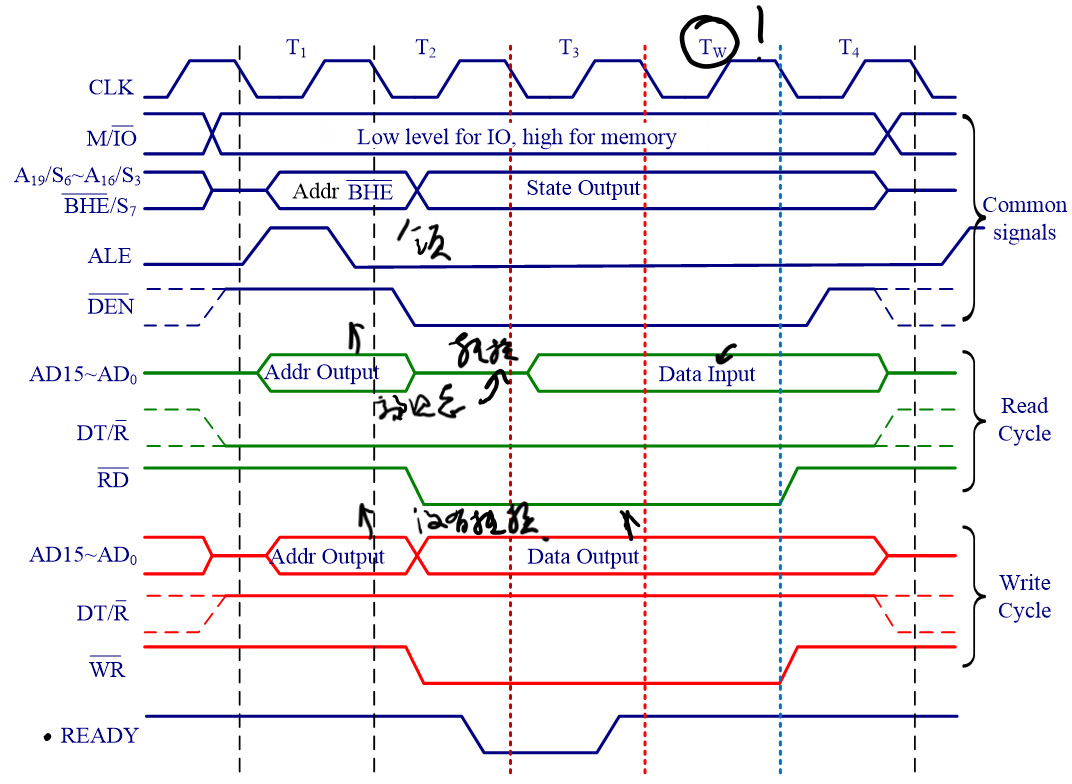
\includegraphics[width=\textwidth]{buscycle.png}
%\end{figure}
8086读周期时序:
在8086读周期内,有关总线信号的变化如下:
\begin{enumerate}
\item M/IO在整个读周期保持有效,当进行存储器读操作时,M/IO为高电平;当进行I/O端口读操作时,M/IO为低电平.
\item A19/S6~A16/S3是在T1期间,输出CPU要读取的存储单元的地址高4位.T2~T4期间输出状态信息S6~S3.
\item BHE/S7在T1期间输出BHE有效信号(BHE为低电平),表示高8位数据总线上的信息可以使用,BHE信号通常作为奇地址存储体的选择信号(偶地址存储体的选择信号是最低地址位A0).T2~T4期间输出高电平.
\item ADl5~AD0在T1期间输出CPU要读取的存储单元或I/O端口的地址A15~A0.T2期间为高阻态,T3~T4期间,存储单元或I/O端口将数据送上数据总线.CPU从ADl5~AD0上接收数据.
\item ALE:在T1期间地址锁存有效信号,为一正脉冲,系统中的地址锁存器正是利用该脉冲的下降沿来锁存A19/S6~A16/S3,ADl5~AD0中的20位地址信息以及BHE.
\item RD在T2期间输出低电平,送到被选中的存储器或I/O接口.要注意的是,只有被地址信号选中的存储单元或I/O端口,才会被RD信号从中读出数据(数据送上数据总线ADl5~AD0).
\item DT/R在整个总线周期内保持低电平,表示本总线周期为读周期.在接有数据总线收发器的系统中,用来控制数据传输的方向.
\item DEN在T2~T3期间输出有效低电平,表示数据有效.在接有数据总线收发器的系统中,用来实现数据的选通.
\end{enumerate}

8086写周期时序总线写操作的时序与读操作时序相似,其不同处在于:
\begin{enumerate}
\item 	
AD15~AD0在T2~T4期间送上欲输出的数据,而无高阻态.
\item WR在T2~T4期间输出有效低电平,该信号送到所有的存储器和I/O接口.要注意的是,只有被地址信号选中的存储单元或I/O端口才会被WR信号写入数据.
\item DT/R在整个总线周期内保持高电平,表示本总线周期为写周期.在接有数据总线收发器的系统中,用来控制数据传输方向.
\end{enumerate}

条件符:
\begin{description}
	\item[CF](Carry Flag): 进位符 set whenever there is a carry out, from d7 after a 8-bit op, from d15 after a 16-bit op
	\item[PF](Parity Flag): 校验符 the parity of the op result’s low-order byte,  set when the byte has an even number of 1s (偶1为1)
	\item[AF](Auxiliary Carry Flag): 辅助进位符 set if there is a carry from d3 to d4, used by BCD-related arithmetic
	\item[ZF](Zero Flag): 零 set when the result is zero
	\item[SF](Sign Flag): 符号符 copied from the sign bit (the most significant bit) after op
	\item[OF](Overflow Flag): 溢出符 set when the result of a signed number operation is too large, causing the sign bit error
\end{description}
控制符:
\begin{description}
	\item[IF] (Interrupt Flag): 中断符 set or cleared to enable or disable only the external maskable interrupt requests
	 
	{\scriptsize
		After reset, all flags are cleared which means you (as a programmer) have to set IF in your program if allow INTR.
	}
	\item[DF] (Direction Flag): 方向符 indicates the direction of string operations
	\item[TF] (Trap Flag): 陷阱符 when set it allows the program to single-step, meaning to execute one instruction at a time for debugging purposes
\end{description}

% %\end{multicols}
\end{CJK}
\end{document}